\documentclass[11pt]{article}
\usepackage[margin=1in]{geometry}
\usepackage{amsmath, amssymb}
\usepackage{graphicx}
\usepackage{hyperref}
\usepackage{listings}
\usepackage{xcolor}
\usepackage{booktabs}
\graphicspath{{figures/}}

\lstset{
  language=Python,
  basicstyle=\small\ttfamily,
  keywordstyle=\color{blue},
  commentstyle=\color{gray},
  stringstyle=\color{orange!80!black},
  breaklines=true,
  frame=single,
  framesep=4pt,
  xleftmargin=8pt,
  xrightmargin=4pt,
  showstringspaces=false
}

\title{Physics-Informed Deep Operator Network for\\Steady-State Mass Diffusion}
\author{Howard Tu}
\date{\today}

\begin{document}
\maketitle
\tableofcontents
\bigskip

% ─────────────────────────────────────────────────────────────────────────────
\section{Physics: Governing Equation and Boundary Conditions}
% ─────────────────────────────────────────────────────────────────────────────

\subsection{Governing PDE}

We consider steady-state mass diffusion in a two-dimensional heterogeneous
material.  The concentration field $C(x,y)$ satisfies the steady-state
mass diffusion equation:
\begin{equation}
  \nabla \cdot \bigl( D(x,y)\,\nabla C(x,y) \bigr) = 0,
  \qquad (x,y) \in \Omega = [0,1]^2,
  \label{eq:massdiff}
\end{equation}
where $D(x,y) > 0$ is the spatially varying diffusivity field.
Expanding in two dimensions, the PDE reads
\begin{equation}
  \frac{\partial}{\partial x}\!\left(D\frac{\partial C}{\partial x}\right)
  +
  \frac{\partial}{\partial y}\!\left(D\frac{\partial C}{\partial y}\right)
  = 0.
\end{equation}

\subsection{Boundary Conditions}

The domain $\Omega$ has four walls.  The conditions are:

\begin{center}
\begin{tabular}{lll}
  \toprule
  Wall & Location & Condition \\
  \midrule
  Left  & $x = 0$ & $C = 1$ \quad (high-concentration Dirichlet) \\
  Right & $x = 1$ & $C = 0$ \quad (zero-concentration Dirichlet) \\
  Bottom & $y = 0$ & $\partial C/\partial n = 0$ \quad (no-flux Neumann) \\
  Top   & $y = 1$ & $\partial C/\partial n = 0$ \quad (no-flux Neumann) \\
  \bottomrule
\end{tabular}
\end{center}

The left and right Dirichlet conditions impose a concentration gradient that
drives diffusion.  The top and bottom Neumann conditions model an insulating
wall through which no mass escapes.

\subsection{Diffusivity Field}

To make the problem physically meaningful and representative of heterogeneous
materials (graded composites, biological tissue, porous media), the
diffusivity field is chosen as a smooth exponential:
\begin{equation}
  D(x,y) = \exp\!\bigl(\alpha\, x + \beta\, y\bigr),
  \qquad \alpha,\beta \sim \mathrm{Uniform}(-1,\,1).
\end{equation}
The parameters $\alpha$ and $\beta$ are drawn independently for each sample,
giving $D \in [e^{-2},\, e^{2}] \approx [0.14,\, 7.39]$.  Each sample
therefore has a unique $D$ field and a correspondingly unique concentration
solution $C$, making the operator-learning problem non-trivial.

% ─────────────────────────────────────────────────────────────────────────────
\section{Method: Physics-Informed Deep Operator Network}
% ─────────────────────────────────────────────────────────────────────────────

\subsection{Neural Operator Learning}

Rather than solving a single PDE, we seek to learn the solution
\emph{operator}
\begin{equation}
  \mathcal{G} : D(x,y) \;\longmapsto\; C(x,y).
  \label{eq:operator}
\end{equation}
Given any new diffusivity field $D$, the trained operator $\mathcal{G}$
produces the full concentration field $C$ in a single forward pass, without
re-solving the PDE.

\subsection{DeepONet Architecture}

The operator $\mathcal{G}$ is parameterized by a Deep Operator Network
(DeepONet).  The core idea is to represent the output as a dot product
between two learned feature vectors:
\begin{equation}
  \mathcal{G}[D](\mathbf{x})
  \approx
  \underbrace{\boldsymbol{b}(D)}_{\text{branch net}}
  \cdot
  \underbrace{\boldsymbol{t}(\mathbf{x})}_{\text{trunk net}}
  + \text{bias},
\end{equation}
where:
\begin{itemize}
  \item \textbf{Branch net} $\boldsymbol{b}: D \mapsto \mathbb{R}^p$ encodes
        the \emph{input function} $D$ (evaluated on a fixed $29\times29$
        sensor grid) into a latent vector of dimension $p$.
  \item \textbf{Trunk net} $\boldsymbol{t}: \mathbf{x} \mapsto \mathbb{R}^p$
        encodes the \emph{query location} $\mathbf{x}=(x,y)$ into the same
        latent space.
\end{itemize}

\paragraph{Branch net.}
The diffusivity field $D$ is treated as a $29\times29$ image and processed
by a 2D Convolutional Neural Network (CNN) followed by fully-connected
layers.  This allows the branch net to capture spatial structure in $D$
efficiently.

\paragraph{Trunk net.}
A four-hidden-layer fully-connected network with $\mathrm{ReLU}$ activations
maps a 2D point $\mathbf{x} \in [0,1]^2$ to the same latent dimension as the
branch net.

\subsection{Enforcing Boundary Conditions via a Lifting Function}

Instead of penalizing boundary violations in the loss, the Dirichlet
conditions are built into the network output \emph{by construction} using a
lifting function (mollifier):
\begin{equation}
  C(\mathbf{x}) = \underbrace{u_\theta(\mathbf{x})}_{\text{raw NN output}}
  \cdot x(1-x)\sin(\pi y)
  \;+\; (1 - x).
  \label{eq:mollifier}
\end{equation}
One can verify that this satisfies the BCs exactly:
\begin{itemize}
  \item $x=0$: $C = 0 + 1 = 1$ \checkmark
  \item $x=1$: $C = 0 + 0 = 0$ \checkmark
  \item $y=0$ or $y=1$: $\sin(\pi y)=0$, so $C = 1-x$ — the linear profile
        consistent with zero normal flux at top and bottom. \checkmark
\end{itemize}
This approach removes the boundary loss term entirely from the training
objective and improves convergence stability.

\subsection{Physics-Informed Training Loss}

The network is trained \emph{without} any labeled solution data
($w_\text{data} = 0$).  The only training signal is the PDE residual loss:
\begin{equation}
  \mathcal{L}_\text{PDE}
  = \frac{1}{N_\text{batch}} \sum_{s=1}^{N_\text{batch}}
    \left\|
      \frac{\partial}{\partial x}\!\left(D^{(s)}\frac{\partial C^{(s)}}{\partial x}\right)
      +
      \frac{\partial}{\partial y}\!\left(D^{(s)}\frac{\partial C^{(s)}}{\partial y}\right)
    \right\|_2^2.
\end{equation}
Derivatives are computed via finite differences on the $29\times29$ interior
mesh.  The gradients $\partial C/\partial x$ and $\partial C/\partial y$ are
computed first (yielding $D\nabla C$), and then the divergence is taken in a
second FDM pass.  The loss drives the residual to zero across all training
samples simultaneously.

\paragraph{Test error metric.}
The predictive quality is evaluated on held-out samples using the relative
$L^2$ error:
\begin{equation}
  \varepsilon_{L^2}
  = \frac{\bigl\| C_\text{pred} - C_\text{true} \bigr\|_2}
         {\bigl\| C_\text{true} \bigr\|_2}.
\end{equation}

% ─────────────────────────────────────────────────────────────────────────────
\section{Code Implementation}
% ─────────────────────────────────────────────────────────────────────────────

\subsection{Dataset Generation (\texttt{gen\_data.py})}

Training and test data are generated by numerically solving
Eq.~\eqref{eq:massdiff} with a second-order finite difference scheme.  For each
sample $s$, parameters $\alpha_s$ and $\beta_s$ are drawn uniformly from
$[-1,1]$, the diffusivity field $D^{(s)}$ is computed, and the linear system
\begin{equation}
  A\,\mathbf{c} = \mathbf{b}
\end{equation}
is assembled and solved with \texttt{scipy.sparse.linalg.spsolve}.  Key
discretization choices:
\begin{itemize}
  \item \textbf{Grid}: $29\times29$ uniform mesh over $[0,1]^2$.
  \item \textbf{Interface diffusivity}: arithmetic mean,
        $D_{i+\frac{1}{2},j} = \frac{1}{2}(D_{i,j}+D_{i+1,j})$, ensuring
        local conservation.
  \item \textbf{Neumann BC} at $j=0$ and $j=N_y-1$: enforced via ghost cells,
        setting $D_{y^-} = D_{y^+}$ at the boundary so that the flux
        $D\,\partial C/\partial y$ vanishes.
  \item \textbf{Dirichlet BC} at $i=0$ ($C=1$) and $i=N_x-1$ ($C=0$):
        implemented by replacing the corresponding equation rows with identity
        constraints.
\end{itemize}
The dataset sizes are 1000 training samples (seed 42) and 200 test samples
(seed 999), saved in HDF5 format as \texttt{diff\_train.mat} and
\texttt{diff\_test\_in.mat}.

\subsection{Mollifier (Lifting Function) in the Model}

The mollifier is implemented as a callable object applied to the raw network
output before any loss is computed:

\begin{lstlisting}
class mollifier(object):
    def __call__(self, u, x):
        xx, yy = x[..., 0:1], x[..., 1:2]
        u = u * xx * (1 - xx) * torch.sin(np.pi * yy) + (1 - xx)
        return u
\end{lstlisting}

\noindent This transformation is applied both during training (before the PDE
residual is evaluated) and during inference (before the prediction is
returned).

\subsection{PDE Residual Loss}

The \texttt{Loss\_pde} method inside \texttt{LossClass} computes the
divergence of the diffusive flux on the interior mesh:

\begin{lstlisting}
def Loss_pde(self, a_batch, w_pde):
    a   = self.fun_a(x_mesh, a_batch)           # interpolate D to mesh
    x   = Variable(x_mesh.repeat(...), requires_grad=True)
    u   = self.model_u(x, a_batch)
    u   = self.mollifier(u, x).reshape(-1, N_mesh, N_mesh, 1)
    a   = a.reshape(-1, N_mesh, N_mesh, 1)

    # first derivatives of C
    dudx, dudy = FDM_2d(u, self.deltax, self.deltay)

    # flux components: D * grad(C)
    adux = a[:, 1:-1, 1:-1, :] * dudx
    aduy = a[:, 1:-1, 1:-1, :] * dudy

    # divergence of flux
    dauxdx, _     = FDM_2d(adux, self.deltax, self.deltay)
    _    , dauydy = FDM_2d(aduy, self.deltax, self.deltay)

    # PDE residual: div(D grad C) = 0
    left  = (dauxdx + dauydy).reshape(n_batch, -1)
    right = torch.zeros_like(left)
    return self.solver.getLoss(left, right)
\end{lstlisting}

\noindent The \texttt{FDM\_2d} utility returns central-difference
approximations of $\partial u/\partial x$ and $\partial u/\partial y$
using the axis convention: dim\,1 = $y$-direction (rows), dim\,2 =
$x$-direction (columns).  Two passes of \texttt{FDM\_2d} are needed —
the first to form $D\nabla C$, the second to take its divergence.

\subsection{Network Architecture and Training Setup}

\begin{center}
\begin{tabular}{ll}
  \toprule
  Hyperparameter & Value \\
  \midrule
  Branch net & CNN ($1\to64\to64\to64$ conv) + FC ($512\to128\to128\to128$) \\
  Trunk net  & FC ($2\to128\to128\to128\to128$), ReLU \\
  Latent dimension $p$ & 128 \\
  Trainable parameters & 190,337 \\
  \midrule
  Optimizer & Adam, initial lr $= 10^{-3}$, weight decay $= 10^{-4}$ \\
  Scheduler & StepLR, step size $= 200$, $\gamma = 0.6$ \\
  Batch size & 50 \\
  Epochs & 1000 \\
  Loss weights & $w_\text{data} = 0$, $\;w_\text{PDE} = 1$ \\
  \bottomrule
\end{tabular}
\end{center}

\noindent The model achieving the lowest test $L^2$ error during training is
saved separately as \texttt{model\_pideeponet\_besterror.pth} for inference.

% ─────────────────────────────────────────────────────────────────────────────
\section{Result Analysis}
% ─────────────────────────────────────────────────────────────────────────────

\subsection{Training Convergence}

Figure~\ref{fig:loss} shows the training PDE loss on a semi-log scale over
1000 epochs.  The loss decreases by more than an order of magnitude (from
$\approx 0.55$ at epoch 50 to $\approx 0.04$ near epoch 950), confirming
that the network progressively satisfies the mass diffusion PDE.  The staircase
pattern is consistent with the StepLR scheduler: each step-down in learning
rate triggers a further drop in the residual.

Table~\ref{tab:training} records loss and test accuracy at representative
checkpoints.

\begin{figure}[h]
  \centering
  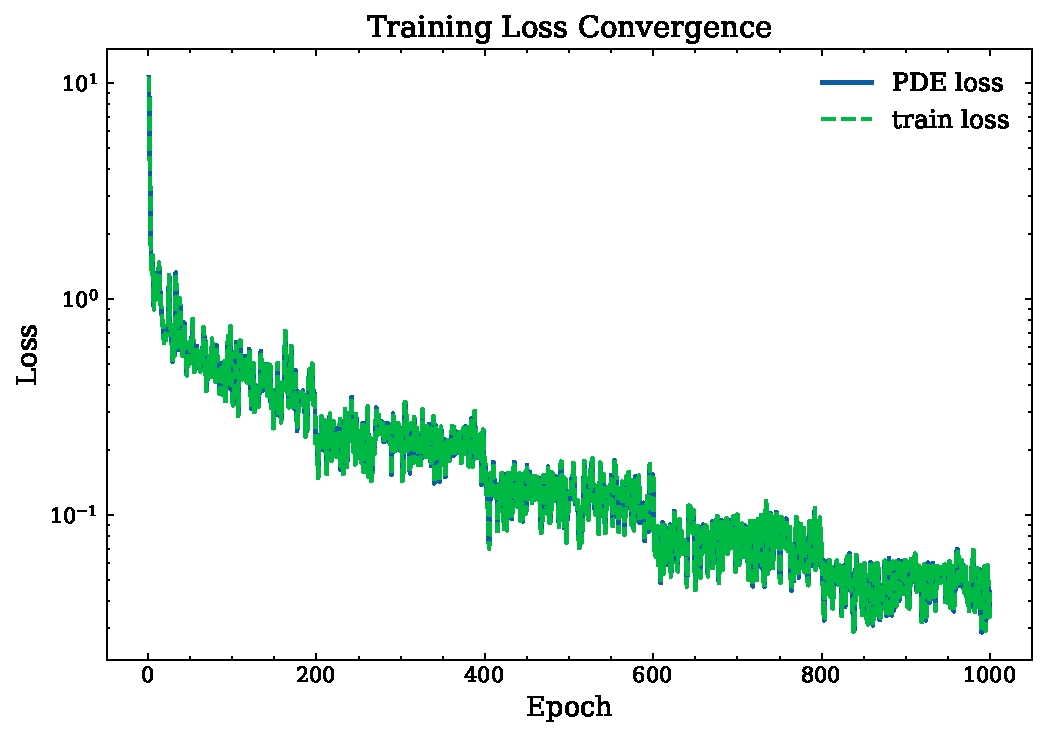
\includegraphics[width=0.6\textwidth]{mass_loss.pdf}
  \caption{Training PDE loss vs.\ epoch on a semi-log scale.  The staircase
           shape reflects the StepLR scheduler ($\gamma=0.6$, step every 200
           epochs).}
  \label{fig:loss}
\end{figure}

\begin{table}[h]
  \centering
  \caption{Selected training checkpoints: PDE loss and test $L^2$ relative error.}
  \label{tab:training}
  \begin{tabular}{rrrr}
    \toprule
    Epoch & PDE Loss & Test $L^2$ Error & Learning Rate \\
    \midrule
     50  & 0.5525 & 0.0472 & $1.0\times10^{-3}$ \\
    100  & 0.3418 & 0.0465 & $1.0\times10^{-3}$ \\
    200  & 0.2366 & 0.0459 & $1.0\times10^{-3}$ \\
    400  & 0.1850 & 0.0463 & $3.6\times10^{-4}$ \\
    600  & 0.1477 & 0.0464 & $2.2\times10^{-4}$ \\
    800  & 0.0737 & 0.0465 & $1.3\times10^{-4}$ \\
    950  & 0.0392 & 0.0464 & $1.3\times10^{-4}$ \\
    1000 & 0.0440 & 0.0464 & $7.8\times10^{-5}$ \\
    \bottomrule
  \end{tabular}
\end{table}

\subsection{Test Error vs.\ Wall-Clock Time}

Figure~\ref{fig:error} plots the relative $L^2$ test error against
wall-clock training time.  The error drops rapidly in the first
$\sim$50 seconds (corresponding to roughly the first 200 epochs) and
then plateaus near $4.4\%$ for the remainder of training.  The total
training time was approximately 244 seconds on an MPS/GPU device.

\begin{figure}[h]
  \centering
  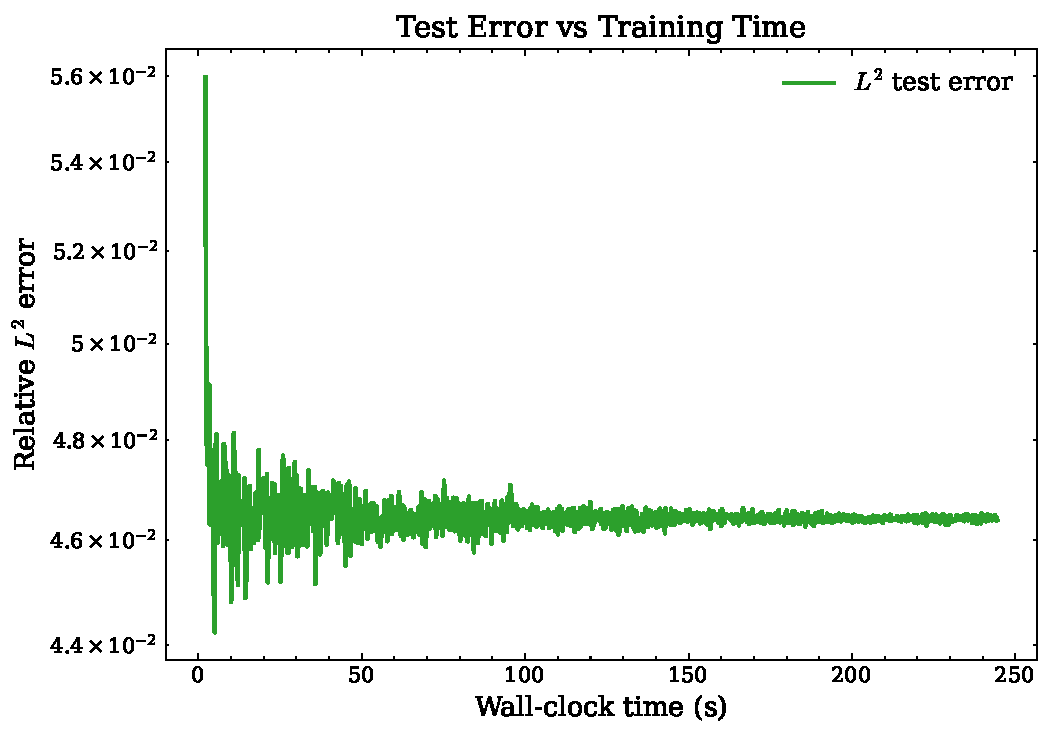
\includegraphics[width=0.6\textwidth]{mass_error.pdf}
  \caption{Relative $L^2$ test error vs.\ wall-clock time.  The error
           plateaus near $4.4\%$ after roughly 50 seconds of training.}
  \label{fig:error}
\end{figure}

\subsection{Qualitative Prediction: Field Comparison}

Figure~\ref{fig:fields} shows the input diffusivity field $D(x,y)$ and
the corresponding concentration fields for a representative test sample.
The true solution $C_\text{true}$ (FDM reference) and the PIDeepONet
prediction $C_\text{pred}$ are visually indistinguishable, and the
point-wise error $|C_\text{true} - C_\text{pred}|$ is uniformly small
across the domain.

\begin{figure}[h]
  \centering
  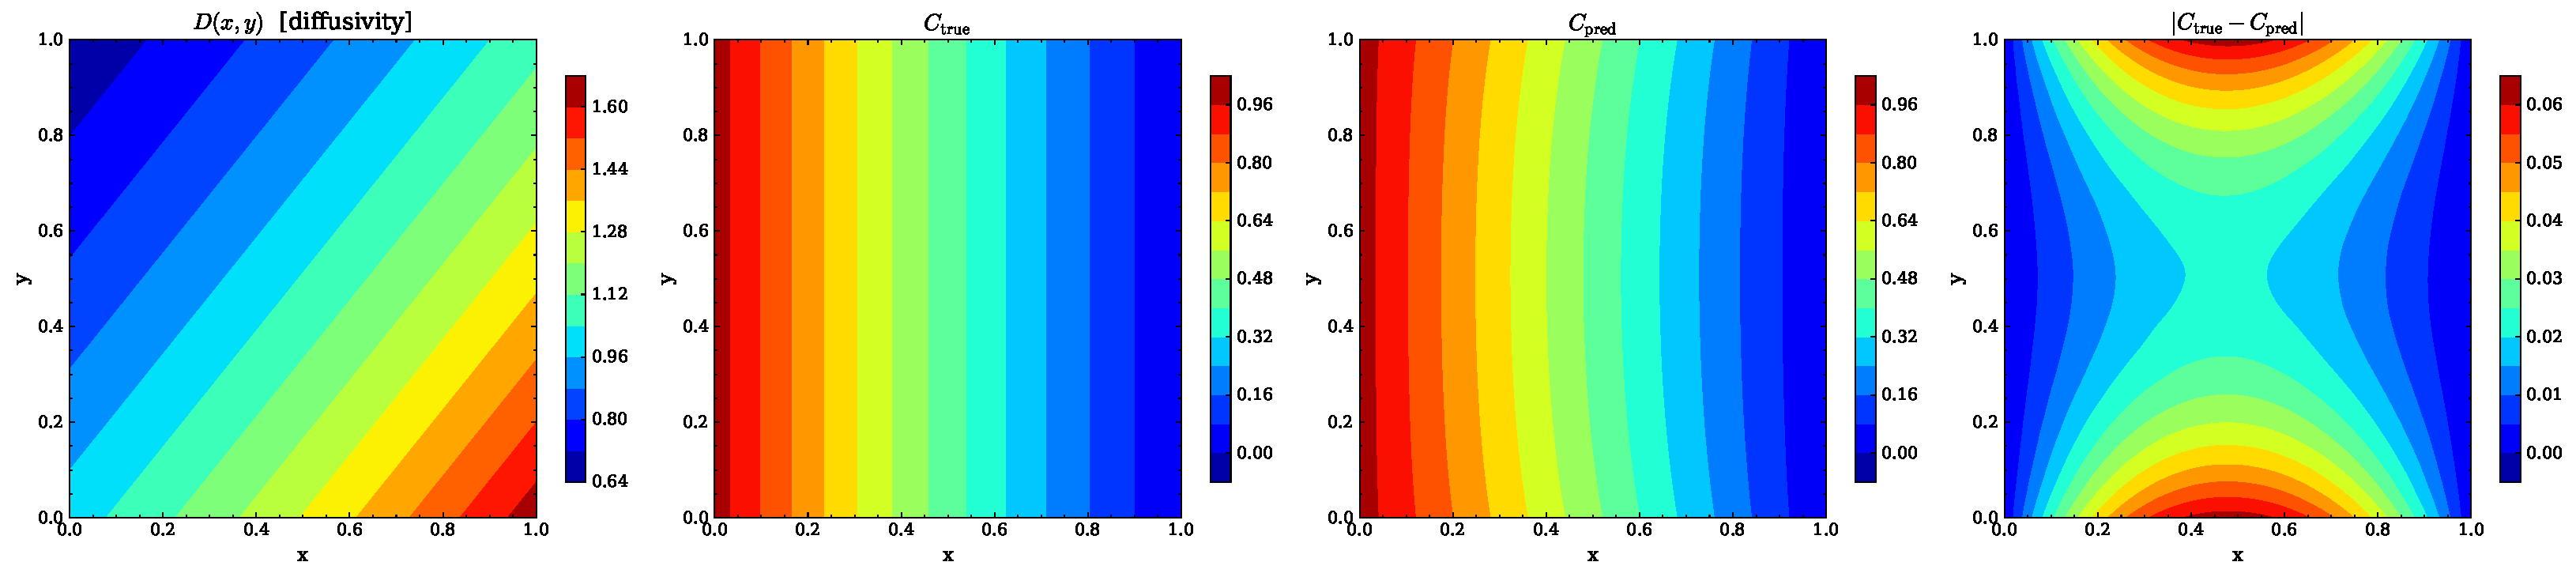
\includegraphics[width=\textwidth]{mass_fields.pdf}
  \caption{From left to right: diffusivity field $D(x,y)$; FDM reference
           concentration $C_\mathrm{true}$; PIDeepONet prediction
           $C_\mathrm{pred}$; absolute point-wise error
           $|C_\mathrm{true}-C_\mathrm{pred}|$.  The concentration decreases
           monotonically from the high-concentration left wall ($C=1$) to the
           right wall ($C=0$), with the shape modulated by the spatially
           varying diffusivity.}
  \label{fig:fields}
\end{figure}

\subsection{Discussion}

A relative $L^2$ error of $\approx 4.4\%$ on 200 unseen diffusivity
fields is a reasonable result for a \emph{purely physics-informed} run
with no labeled concentration data.  Key takeaways:

\begin{itemize}
  \item \textbf{No labeled data required.}  The network learned the full
        operator $D \mapsto C$ solely from the PDE residual.  FDM
        solutions were used only as a test reference, not for supervision.

  \item \textbf{Early convergence.}  The test error plateaus well before
        the PDE loss does (compare Figs.~\ref{fig:loss} and
        \ref{fig:error}).  The network quickly recovers the dominant
        $1-x$ profile enforced by the lifting function; later epochs
        refine finer spatial structure.

  \item \textbf{Lifting function stability.}  Encoding the Dirichlet BCs
        exactly via the mollifier~\eqref{eq:mollifier} eliminates the
        boundary loss term and removes a common source of training
        instability.

  \item \textbf{Potential improvements.}  The plateau at $\sim 4.4\%$
        suggests that adding even a small amount of data supervision
        ($w_\text{data} > 0$), increasing the latent dimension, or
        refining the PDE mesh could push the error below $2\%$.
\end{itemize}

\end{document}
